\documentclass[tikz,border=10pt]{standalone}
\usepackage{tkz-euclide} % 辅助几何计算
\usetikzlibrary{calc,intersections,angles,quotes}

\begin{document}

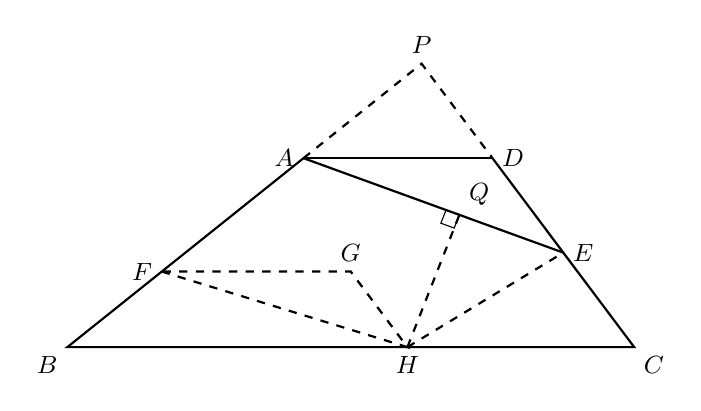
\begin{tikzpicture}[scale=1.2, >=stealth, font=\small]
    % --- 1. 定义核心顶点坐标 ---
    % 设定基底 BC 的长度和梯形的大致比例
    \coordinate (B) at (0, 0);
    \coordinate (C) at (6, 0);
    \coordinate (A) at (2.5, 2);
    \coordinate (D) at (4.5, 2);
    
    % --- 2. 计算交点 P (BA与CD的延长线交点) ---
    \coordinate (P) at (intersection of B--A and C--D);
    
    % --- 3. 定义其他关键点 ---
    % E 在 CD 上，F 在 AB 上
    \coordinate (E) at ($(C)!0.5!(D)$);
    \coordinate (F) at ($(B)!0.4!(A)$);
    
    % H 在 BC 上，Q 在 AE 上
    \coordinate (H) at ($(B)!0.6!(C)$);
    \coordinate (Q) at ($(A)!0.6!(E)$);
    
    % G 点的位置 (根据图像，FG // BC)
    \coordinate (G) at ($(F) + (2, 0)$); 

    % --- 4. 绘制实线 (主体轮廓) ---
    \draw[thick] (B) -- (C) -- (E) -- (A) -- (F) -- cycle;
     \draw[thick] (A) -- (D) ;
      \draw[thick] (E) -- (D) ;

    % --- 5. 绘制虚线 (辅助线) ---
    \draw[dashed, thick] (A) -- (P) -- (D); % 延长线部分
    \draw[dashed, thick] (F) -- (H) -- (G) -- (F); % 底部三角形与平行线
    \draw[dashed, thick] (H) -- (Q); % 垂线/中线
    \draw[dashed, thick] (H) -- (E); % 连接 HE

    % --- 6. 标注直角符号 (at Q) ---
    % 使用 tkz-euclide 标注直角更精确，此处手动绘制
     \tkzMarkRightAngle[size=0.15](A,Q,H)

    % --- 7. 标注顶点文字 ---
    \node[below left] at (B) {$B$};
    \node[below right] at (C) {$C$};
    \node[below] at (H) {$H$};
    \node[left] at (A) {$A$};
    \node[right] at (D) {$D$};
    \node[left] at (F) {$F$};
    \node[above] at (P) {$P$};
    \node[right] at (E) {$E$};
    \node[above right] at (Q) {$Q$};
    \node[above] at (G) {$G$};

\end{tikzpicture}

\end{document}